%File: submission_v13.tex --- AAAI-27 anonymous submission (v12-review response: statistical vocabulary, formulation wording, typography)
% "An Empirical Analysis of Transfer for Dynamic Path Planning"
% Built on the official AAAI-27 author kit (aaai2027.sty, TemplateVersion 2027.1).
\documentclass[letterpaper]{article} % DO NOT CHANGE THIS
\usepackage[submission]{aaai2027}  % DO NOT CHANGE THIS
\usepackage[hyphens]{url}  % DO NOT CHANGE THIS
\usepackage{graphicx} % DO NOT CHANGE THIS
\urlstyle{rm} % DO NOT CHANGE THIS
\def\UrlFont{\rm}  % DO NOT CHANGE THIS
\usepackage{natbib}  % DO NOT CHANGE THIS AND DO NOT ADD ANY OPTIONS TO IT
\usepackage{caption} % DO NOT CHANGE THIS AND DO NOT ADD ANY OPTIONS TO IT
\frenchspacing  % DO NOT CHANGE THIS
%
% Recommended for better-looking tables
\usepackage{booktabs}
\usepackage{amsmath}
%
\pdfinfo{
/TemplateVersion (2027.1)
}
\setcounter{secnumdepth}{0}

% Custom macros

\title{An Empirical Analysis of Transfer for Dynamic Path Planning}
\author{
    Anonymous Submission
}
\affiliations{
}

\begin{document}

\maketitle

\begin{abstract}
We study the dynamic path planning problem, where an agent plans a route among moving obstacles, and ask whether heuristics learned on training maps transfer to unseen environments, zero-shot or from a few labeled target maps. Within budgeted time-expanded A\textsuperscript{*}, and with the right training formulation and planner integration, a single learned heuristic transfers zero-shot to new maps drawn from six procedural continuous dynamic suites. It was selected on development maps, frozen before the confirmation maps were generated, and given no future-motion input (the planner retains the exact obstacle trajectories). Yet it improves success over a geometric anchor while expanding 73--95\% fewer nodes on maps both methods solve. Selected discrete-grid experiments show a smaller, rank-only effect. In static few-shot experiments with one labeled target map, low-rank adaptation preserves success better than full fine-tuning; with sixteen maps, full fine-tuning searches more efficiently at similar success. In a matched-label factorial, full fine-tuning and from-scratch training degrade when a fixed label count is drawn from very few distinct worlds; spreading that count across more worlds prevents the degradation in the tested cells. No architecture is uniformly best across the tested formulations: MLPs, recurrent models, Hierarchical Reasoning Models, and U-Nets each lead in different settings, and hierarchy-specific gains do not persist.
\end{abstract}

\section{Introduction}

Dynamic path planning searches over both configuration and time: when obstacles move, a planner must consider waiting, detouring, and timing, and the search space grows accordingly \citep{silver2005cooperative,phillips2011sipp}. The geometric admissible heuristics that make A\textsuperscript{*} \citep{hart1968astar} efficient on static maps (the \emph{anchor} baselines of this paper) ignore exactly these temporal effects, so search effort grows sharply with moving obstacles. Learned heuristics can reduce search effort \citep{arfaee2011bootstrap,bhardwaj2017sail,yonetani2021neuralastar}, but a deployed planner benefits only if a heuristic trained on one set of maps remains useful on maps it has never seen. We study zero-shot and few-shot transfer of learned heuristics to unseen environments for dynamic path planning. Budgeted time-expanded A\textsuperscript{*} serves throughout as a controlled measurement substrate; we do not propose it as a replacement for dedicated dynamic planners.

We organize the experiments around three factors: the training formulation, the way the prediction enters the planner, and the distribution of target supervision. Each factor is evaluated first on static suites, then under deterministic dynamics. Comparisons use matched controls throughout: aware/blind pairs (with and without future-motion input) otherwise matched, identical weights under different integrations, anchor-calibrated budgets, and map-level paired inference \citep{henderson2018matters,agarwal2021precipice,pineau2021reproducibility}. Confirmatory comparisons, units, and criteria are specified before test evaluation. Across the tested settings, the training formulation, planner integration, and supervision distribution explain the observed transfer outcomes more consistently than model family.

Our contributions are:
\begin{itemize}
    \item \textbf{Dynamic zero-shot transfer with one fixed learned heuristic.} A single U-Net heuristic improves success on all six dynamic suites of a 50-map-per-suite confirmation cohort ($+0.18$ to $+0.84$) and cuts matched expansions by 73--95\% on jointly solved maps. Every paired map-level CI excludes zero and every exact McNemar test survives BH correction ($q \leq 0.0039$). The model was development-selected, frozen before the confirmation cohort was generated, and given no future-motion input. Three suites are held out from training: one distinct topology and two parameter/scale shifts; the remaining three draw disjoint maps from trained families.
    \item \textbf{Training formulation and planner integration determine whether transferred predictions reduce search.} Changing the coupled input--target--output formulation yields useful recurrent-model guidance where the scalar formulation collapses; changing only the planner integration makes an inert discrete residual useful; and sharing one search state turns an exact oracle from a six-map loss into a six-map win. A negative planning result therefore does not isolate the model unless target and search interface are held fixed.
    \item \textbf{At fixed label count, distinct-world coverage controls the observed held-out degradation in the tested matched-label factorial.} With scarce static supervision, low-rank adaptation preserves the transferred prior while full fine-tuning is unstable; with more supervision, full fine-tuning often overtakes it on search effort at near-parity success. The largest held-out losses occur for full fine-tuning and from-scratch training when a fixed label count comes from very few distinct worlds; spreading the same labels across more worlds prevents those losses in the tested cells, and targeted redraws preserve the positive direction. Low-rank adaptation degrades least often and least severely, though one redraw LoRA cell has a harmful interval excluding zero.
\end{itemize}
Weighted A\textsuperscript{*}, SIPP, and an external MovingAI test bound the scope. Under the tested weighted-A\textsuperscript{*} grid, the learned heuristic keeps a success advantage only on spiral, with lower matched expansions on four suites and higher path cost on two. Unbudgeted safe-interval planning (SIPP) solves every instance feasible under the implemented collision model optimally, and the zero-shot success advantage does not reproduce in a small MovingAI-derived boundary test (analyzed post hoc below). Future-window inputs, adapter interpolation, and hierarchy-specific depth add no consistent value. A restricted-observation heuristic with one Bellman backup and frozen scale calibration beats a complete-map comparator on expansions.

\begin{figure*}[t]
\centering
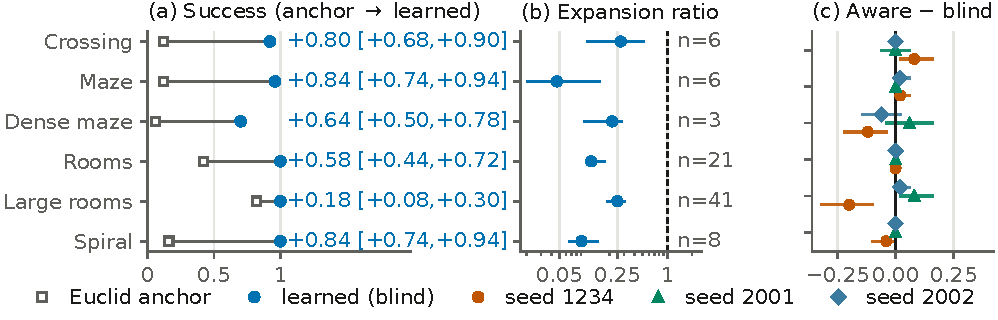
\includegraphics[width=0.98\textwidth]{figures/fig_dynamic_headline.pdf}
\caption{Dynamic zero-shot transfer of the fixed blind U-Net (no future-motion input) on the 50-map-per-suite confirmation cohort (held out from training: crossing, a distinct topology, and dense maze/large rooms, parameter/scale shifts; maze, rooms, and spiral use trained generators with disjoint maps). (a) Anchor and learned success per suite; labels: paired mean delta with map-level 95\% CI (all six exclude zero; marginal). (b) Matched-solved expansion ratios, conditional on joint success (log axis, map-level 95\% CIs); $n$ = jointly solved count (dense maze $n{=}3$ descriptive). (c) Aware$-$blind success differences for the three training pipelines; the large-rooms cell flips sign.}
\label{fig:dynamic}
\end{figure*}

\section{Problem Formulation and Learned-Heuristic Interfaces}

\textbf{Planning problems.} In the continuous setting, a point robot plans on a probabilistic roadmap \citep[PRM;][]{kavraki1996prm} built over a square world of side length $L{=}1.0$ ($2.0$ for the large-room family). Units are abstract. Each roadmap has 192 nodes (start, goal, and 190 sampled free-space nodes) with $k{=}7$ nearest-neighbor candidate edges per node (doubled for start and goal, then symmetrized; appendix). Edges are validated by sampled collision checks at resolution $0.01L$, and unconnected worlds are rejected. Static search states are roadmap nodes, edge costs are Euclidean lengths $\ell(e)$, and the anchor heuristic is Euclidean distance to the goal, $h_0(v) = \lVert x_v - x_g \rVert$.

In the dynamic setting, obstacles move on deterministic trajectories and the search state is a pair $(v,t)$ of node and discrete time step of duration $\Delta t$. The planner may traverse an edge, taking $\tau(e) = \lceil \ell(e) / (v_{\mathrm{agent}} \Delta t) \rceil$ steps ($v_{\mathrm{agent}}$: agent speed), or wait one step. Transitions are validated against the obstacle trajectories by collision checks sampled along the edge (moves) or across the time interval (waits). Cost is arrival time in steps, search runs to a horizon $t_{\max}$, and the anchor is the travel-time lower bound $h_0(v,t) = \lVert x_v - x_g \rVert / (v_{\mathrm{agent}} \Delta t)$, constant in $t$, so anchor and cost share units.

In the discrete setting, agents plan on occupancy grids of $20{\times}20$ to $256{\times}256$ cells with Manhattan distance as the anchor and an analogous capped residual target (appendix).

\textbf{Supervision targets.} The exact cost-to-go $h^{*}$ comes from graph Dijkstra on the static roadmap and from backward space--time Dijkstra over $(v,t)$ dynamically. The regression target is the normalized anchor residual $\bar\delta^{*}(s) = \mathrm{clip}\!\left(h^{*}(s) - h_0(s),\, 0,\, c\,T\right)/T$. Here $T$ is the normalization scale: $T{=}L$ statically, and dynamically $T = L/(v_{\mathrm{agent}}\Delta t)$, the map-crossing time in steps, identical across dynamic suites by construction. The cap $c{=}4.0$ is in normalized units, and unreachable states are masked from the loss. Scalar models predict $\bar\delta_\theta$ from per-node feature tokens. Field models map an eight-channel input raster (appendix) to a goal-conditioned residual raster sampled at node positions. At integration the prediction is rescaled: $\hat h_\theta(s) = h_0(s) + T \cdot \mathrm{clip}(\bar\delta_\theta(s), 0, c)$.

\textbf{Planner integrations.} Under \emph{additive} integration the planner orders states by $f(s) = g(s) + \hat h_\theta(s)$, sacrificing admissibility for guidance. Empirical path-cost ratios are reported wherever additive integration is used. The classical control is weighted A\textsuperscript{*} \citep{pohl1970}, which orders states by $f(s) = g(s) + w_h\, h_0(s)$ with a per-suite success-tuned inflation $w_h$. Under \emph{focal (rank-only)} integration \citep{pohl1970,pearl1982semiadmissible}, the anchor priority $f_0(s) = g(s) + h_0(s)$ defines the band $\mathrm{FOCAL}_w = \{ s \in \mathrm{OPEN} : f_0(s) \leq w \cdot \min_{u \in \mathrm{OPEN}} f_0(u) \}$, and the learned prediction orders expansions only within the band. At $w{=}1.0$ the learned score merely breaks ties among minimum-priority states, preserving the anchor's path-cost optimality when search completes (finite budgets can still change success).

In the restricted-observation study, one inference-time Bellman backup over a radius-bounded local subgraph turns learned exit values into the heuristic (scale calibrated once on a disjoint block).

\textbf{Transfer protocol.} Zero-shot transfer applies a trained-and-fixed heuristic to unseen maps (held-out suite distributions where applicable) and throughout means no target-label training or adaptation. Selecting which trained heuristic to deploy (\emph{provider} selection), where it occurs, uses a disjoint development cohort and is disclosed. Few-shot adaptation draws $K$ labeled target maps and compares low-rank adaptation \citep[LoRA;][]{hu2021lora} (rank 8 for the HRM, rank 24 for the ON-LSTM's wider hidden layer), full fine-tuning, and training from scratch. LoRA and full fine-tuning start from the same trained checkpoint. Scratch uses the same architecture and schedule from random initialization.

\section{Experimental Setup}

\textbf{Environment families.} A \emph{family} is a procedural map generator; a \emph{suite} is a named evaluation condition; a \emph{world} is one sampled environment (interchangeably, a \emph{map}). Continuous worlds come from our procedural generator (specification tables in the appendix; code in the anonymized artifact archive). The static hard families are wall constructions---\emph{maze}/\emph{dense maze} (corridor mazes; the dense variant narrows gaps to $0.115L$), \emph{rooms}/\emph{large rooms} (partition walls with doorways; the large variant doubles the side length), \emph{spiral}, and \emph{bugtrap}. Static training uses the maze, rooms, and spiral families; dense maze, bugtrap, and large rooms are held out from training (bugtrap: distinct topology; dense maze/large rooms: gap- and scale-shifted variants of trained generators).

Dynamic suites add 3--5 moving circular obstacles (\emph{patrollers}) per world that sweep line segments with triangle-wave motion (radius 0.055--0.080$L$, span 0.36--0.50$L$, period 0.14--0.30 of the horizon; per-suite parameters in the appendix). A \emph{crossing} open-arena suite serves as a timing control. \emph{Dynamic training draws worlds only from the dynamic maze, rooms, and spiral families; dynamic dense maze, crossing, and large rooms are held out from training}: crossing is a distinct open-arena topology; dense maze narrows corridors and adjusts patrollers; large rooms doubles the scale and speeds the agent. No learned model observes a test world during training. Evaluation cohorts come from disjoint seed ranges, checked by world fingerprints.

\textbf{Models.} Scalar models consume per-node token sequences (62 tokens of 16 dimensions; appendix) and include an MLP, an LSTM \citep{hochreiter1997lstm}, an ON-LSTM \citep{shen2019onlstm}, and a Hierarchical Reasoning Model \citep[HRM;][]{wang2025hrm} with an adaptive-computation port \citep{graves2016act,banino2021pondernet}. Field models consume the eight-channel $64{\times}64$ raster and include a FiLM-conditioned U-Net \citep{ronneberger2015unet,perez2018film}, a field HRM, and a field ON-LSTM (parameter counts in the appendix). Dynamic variants append $W$ future-occupancy channels ($W{=}8$ aware = ground-truth occupancy at offsets $t{+}1,\ldots,t{+}8$; $W{=}0$ blind). Unless a specific experiment states otherwise, the continuous residual models share one AdamW recipe on a smooth-L1 loss over the capped normalized residual (optimizer constants and architecture tables in the appendix; complete constructors in the artifact). Within each direct architecture comparison, models are trained under one matched recipe on identical data.

\textbf{Evaluation.} Each suite is evaluated at a per-suite expansion budget selected by anchor-only calibration: the budget from a fixed candidate grid whose anchor success is closest to pre-specified targets (evenly spaced in $[0.45, 0.70]$; ties smaller) is chosen before any learned method is compared. The smallest selected budget is the \emph{binding} budget, the primary operating point. The coarse budget grid means realized anchor success at calibration can fall outside the target band (0.05--0.75 dynamic, 0.25--0.62 static; calibration and confirmation rates in the appendix). Static calibration shares worlds with evaluation (anchor-only, never touching learned outcomes; disclosed). The dynamic 50-map-per-suite cohort and the 144-map restricted-observation cohort are \emph{confirmation} cohorts: their budgets were frozen before the cohorts were generated.

Success means reaching the goal within the budget. Appendix success-vs-budget curves up to $4\times$ binding mitigate single-threshold dependence. Search effort is the \emph{matched-solved expansion ratio}: the median over jointly solved maps of the per-map ratio of learned to anchor expansions. Because it conditions on joint success, it can favor methods that solve only easier maps. Success is therefore reported first, with path-cost ratios reported separately (appendix).

\textbf{Statistics.} Success comparisons use paired McNemar tests with Benjamini--Hochberg correction within each experiment's set of suites (adjusted values reported as $q$). Interval estimates are percentile bootstraps (10{,}000 resamples) whose resampling unit is the evaluation map; repeated adaptation or model seeds are averaged within maps before resampling; quoted intervals reflect map uncertainty conditional on the evaluated seeds. Per-suite bootstrap intervals (as in Figure~\ref{fig:dynamic}) are marginal. The corrected McNemar tests are primary (full policy in the appendix). Method-versus-method claims use direct map-paired contrasts. Unless noted, continuous experiments use one primary training seed. The dynamic result adds two retrained pipelines.

\section{Dynamic Zero-Shot Transfer}

\textbf{Setting and fixed-model protocol.} The dynamic experiment trains on the dynamic maze, rooms, and spiral families and evaluates on all six dynamic suites---three sharing a training generator (disjoint maps) and three held out as above (dense maze, crossing, large rooms). The training run keeps 53 usable worlds of 72 candidates (24 drawn per family; usability rules and exact label counts in the appendix). The original 20-map-per-suite cohort served as \emph{development} data: on it we selected the field U-Net \emph{blind} twin and froze its checkpoint, additive integration, and per-suite budgets. The 50-map-per-suite \emph{confirmation} cohort was then generated from a pre-specified seed range, map-disjoint by fingerprint check, with no further choices. Selection still happened, on development data. The protocol protects only the confirmation cohort. The space--time planner and collision checker always use the true deterministic trajectories when validating $(v,t)$ transitions, so the aware/blind ablation changes only the heuristic's input.

\textbf{Confirmation result.} On the confirmation cohort, the fixed blind U-Net raises success on all six suites: deltas $+0.18$ to $+0.84$, every paired map-level 95\% CI excluding zero (exact McNemar $q \leq 0.0039$; every discordant map favors the learned heuristic). Matched expansion-ratio medians are 0.047--0.273, a 73--95\% effort reduction on jointly solved maps (Figure~\ref{fig:dynamic}; joint counts 3--41 per suite). On jointly solved maps the anchor's paths are optimal (admissible anchor; verified), and learned mean suboptimality spans 1.000--1.216 per suite, largest on crossing (anchor-joint maps; the control table's joint sets differ; appendix). Gains on the three held-out suites ($+0.80$ crossing, $+0.64$ dense maze, $+0.18$ large rooms) show transfer under topology and parameter/scale shift. The remaining three suites show map-level generalization within trained families.

\textbf{Independent retraining robustness.} Two additional full training pipelines with independent seeds (2001, 2002) reproduce the success pattern on the same confirmation cohort. They used a larger world-collection budget (139 and 149 usable worlds versus 53; appendix): seed and data scale vary together. Across the three pipelines, 17 of 18 pipeline--suite paired CIs exclude zero (deltas $+0.10$ to $+0.88$; the exception is seed 2001's near-ceiling large-rooms cell, anchor 0.82). Effort magnitudes are stable across pipelines on three suites (medians 0.047--0.135) and pipeline-variable on the other three (0.216--0.625), quoted as across-pipeline ranges there. The retrained models are evaluated on the same 50 maps (retraining robustness, not cohort replication).

\textbf{Tuned weighted A\textsuperscript{*} control.} Because the anchor is deliberately simple, we also compare against weighted A\textsuperscript{*} ($w_h h_0$), success-tuned per suite over $w_h \in \{1.1, 1.2, 1.5, 2, 3, 5\}$ on the development cohort (rule frozen in advance: highest success, ties smaller). The tuned weights are evaluated once on the confirmation cohort. The control was specified after the learned results were known, and tuning touched only development data (appendix). The comparison yields a three-way tradeoff rather than dominance (Table~\ref{tab:wastar-main}). \emph{Success:} no BH-corrected success difference is detected on five suites (at most one discordant map on four; crossing's four-map weighted advantage has $q{=}0.375$ under the exact McNemar policy). The learned heuristic holds the one BH-significant advantage, on spiral ($+0.30$ $[+0.18,+0.42]$; 15/0 discordant, $q{=}3.7\times10^{-4}$). \emph{Effort:} learned-to-weighted expansion medians are below parity everywhere, with the marginal 95\% interval excluding parity on four of six suites (0.217--0.728); crossing and dense-maze intervals include parity (descriptive---the corrected success tests carry the inferential policy). \emph{Path quality:} on jointly solved maps, the additive learned heuristic pays a premium over tuned inflation on crossing ($+0.156$ $[+0.116,+0.200]$) and large rooms ($+0.080$ $[+0.058,+0.105]$), both paired intervals excluding zero. The other four suites stay within $\pm 0.005$, intervals covering zero.

Because three suites selected the grid maximum $w_h{=}5$, we also ran a disclosed post-hoc extension to $w_h \in \{7, 10\}$ (design frozen before execution). Five selections are unchanged, and spiral's development success stays 0.80, so its learned advantage is robust to the tested extension. Dense maze re-selects $w_h{=}7$, changing its point estimates but no inferential conclusion: success 0.74 versus 0.70 against both the frozen rows and the learned arm (exact $p \geq 0.5$), effort intervals covering parity, path quality within $\pm 0.007$ (appendix).

\begin{table*}[t]
\centering
\small
\begin{tabular}{lcccccc}
\toprule
Suite & $w_h$ & Success learned & Success WA* & Expansions learned/WA* [95\% CI] ($n$) & Subopt.\ learned & Subopt.\ WA* \\
\midrule
Crossing & 1.5 & 0.92 & 1.00 & 0.825 [0.531, 1.167] (46) & 1.164 & 1.008 \\
Maze & 5 & 0.96 & 0.96 & 0.601 [0.440, 0.835] (47) & 1.013 & 1.017 \\
Dense maze & 5 & 0.70 & 0.70 & 0.982 [0.823, 1.089] (34) & 1.008 & 1.006 \\
Rooms & 3 & 1.00 & 0.98 & 0.554 [0.439, 0.798] (49) & 1.019 & 1.015 \\
Large rooms & 1.5 & 1.00 & 0.98 & 0.728 [0.536, 0.966] (49) & 1.083 & 1.003 \\
Spiral & 5 & \textbf{1.00} & 0.70 & 0.217 [0.183, 0.312] (35) & 1.014 & 1.013 \\
\bottomrule
\end{tabular}
\caption{Fixed learned heuristic versus per-suite success-tuned weighted A\textsuperscript{*} (original grid), confirmation cohort at binding budgets. Expansions: median learned-to-weighted ratio on the $n$ jointly solved maps [map-bootstrap 95\% CI]. Subopt.: mean arrival over optimal arrival on the same jointly solved maps (paired intervals in text). Bold: the only BH-significant success difference (exact McNemar $q{=}3.7\times10^{-4}$; crossing's four-map gap $q{=}0.375$). A disclosed post-hoc grid extension re-selects $w_h{=}7$ on dense maze but changes no inferential conclusion (success 0.74 vs.\ 0.70, $p \geq 0.5$; appendix).}
\label{tab:wastar-main}
\end{table*}

\textbf{Unbudgeted SIPP nearly saturates the substrate.} We also implemented discrete-time SIPP \citep{phillips2011sipp} on the identical substrate with the same collision predicates and the anchor heuristic. As a hard correctness gate, its outcome (earliest arrival or infeasibility) matches backward space--time Dijkstra on all 300 confirmation instances. Under the implemented sampled-collision model, unbudgeted SIPP therefore solves every feasible instance optimally. Its per-suite success, 0.94--1.00, equals the substrate's feasibility ceiling exactly, with small expansion counts in its own interval-state unit (medians 80--290; never merged with $(v,t)$ expansions). Wall times: SIPP 0.9--1.8\,s per map (full-cohort means); learned 1.18\,s end-to-end (1.02\,s table $+$ 0.15\,s search; components rounded) and weighted A\textsuperscript{*} 0.23\,s on the timing sample (different protocols; appendix). This confines the learned result to budgeted time-expanded search: it does not outperform a dedicated dynamic planner on this deterministic substrate (appendix table).

\textbf{External-geometry boundary.} To test the claim beyond our own generators, six MovingAI maps \citep{sturtevant2012movingai} (three street, three dungeon) were converted to the canonical substrate: 64$\times$64 occupancy, rectangle-decomposed obstacles, and the trained maze-family patroller dynamics. The heuristic was then evaluated under the frozen calibration/tuning protocol. One dungeon map yields no usable instances, so five maps contribute (appendix).

The success advantage does not reproduce in this boundary test. The learned heuristic does not beat the anchor on either group (deltas $-0.08$). On dungeon instances it loses to tuned weighted A\textsuperscript{*} ($-0.28$, 0/7 discordant, exact $p{=}0.016$; instance-level, unadjusted, nested in two maps) and expands more nodes (matched ratio 2.20 $[1.25, 6.36]$). It pays path-quality premiums with intervals excluding zero on both groups. Only the street-map matched-effort advantage over the anchor survives (0.48 $[0.28, 0.64]$). The zero-shot success claim is therefore bounded to the procedural families and their tested shifts. A post-hoc residual analysis (appendix) ties the failure to degraded prediction: correlation falls from 0.73--0.98 on the procedural suites to 0.24--0.39 on the converted maps, error roughly doubles, and the bias turns positive, so the nonnegative additive interface inflates the wrong regions. An exploratory within-group adaptation study is in the appendix.

\textbf{Future-window inputs provide no consistent benefit.} The primary model is already the blind twin; the aware twin adds the eight future-occupancy input channels (first layer only; architecture and training otherwise matched). On the confirmation cohort the contrast is suite-dependent in both directions and unstable across pipelines. Of 18 contrasts, the paired interval excludes zero for the aware twin in two, the blind twin in two, and neither in fourteen. No suite's interval excludes zero in the same direction for more than one pipeline (large rooms flips sign). The canonical pipeline also trained on fewer worlds, but the two collection-matched retrains still disagree (Figure~\ref{fig:dynamic}(c); appendix). After full fine-tuning at $K{=}16$, eight of the nine target$\times$architecture aware$-$blind success differences are non-positive (the ninth includes zero). We report a failure to observe a systematic future-window benefit under deterministic dynamics---not equivalence, and not harm. Stochastic motion is untested.

\section{Effects of Supervision Target and Planner Integration}

\textbf{Static family transfer.} On the six calibrated static suites, the transferred field HRM solves 0.75--1.00 of test maps against anchor success of 0.25--0.58 (BH-adjusted $q \leq 0.025$ on four suites, the other two corrected-significant only for other learned arms; matched expansion ratios 0.521--0.850; appendix). Three of six suites are held out from training as above, and models trained on data pooled across the three source families (\emph{pooled} models) improve success on every held-out suite before any target labels.

\textbf{Supervised target.} On the calibrated hard static maps, a pooled ON-LSTM scalar residual model raises hard-maze success from 0.525 to 1.000 over the anchor ($q=4.3\times10^{-11}$). The scalar HRM, under the same recipe and data, instead collapses to a constant prediction at the residual cap and merely matches the baseline (lower learning rates and a soft cap reproduce the collapse). Retaining the HRM while changing input representation, supervised target, and output head to the raster residual field raises hard-maze success from that run's 0.625 anchor to 0.975 ($q=3.4\times10^{-4}$). A later experiment shows a well-trained scalar HRM is also viable (ratios 0.427--0.822). The failure is therefore formulation-specific rather than intrinsic to the HRM. The field intervention changes input, target, and output head together, so it does not isolate which component matters.

\textbf{Planner integration.} The preferred integration differs between the two tested substrates. On continuous roadmaps, additive residuals exploit the gap the Euclidean anchor leaves (the field-HRM ratios above, at empirical path-cost ratios of roughly 1.02--1.14), while rank-only variants stay closer to plain anchor search. On discrete grids the learned signal is accurate: the pooled residual correlates 0.987--0.994 with the true residual across map sizes. But its magnitude is scale-flat (predicted/true mean 0.73 to 0.19 as maps grow), and every additive arm in a 22-suite transfer evaluation (appendix) is at or below its matched baseline. We then reuse the \emph{same} trained predictions only to rank expansions inside a $w{=}1.0$ focal band: expansions fall 6--15\% with no observed success regression \citep{chrestien2023rank}. Changing only the integration recovered the ordering signal. We interpret the cross-substrate pattern (additive helps against a looser anchor, ranking against a tighter one) as a supported hypothesis. Anchor tightness itself is not directly measured.

\textbf{Oracle integration control.} An oracle control removes model-estimation error: exact optimal values rank expansions inside a $w{=}1.10$ focal band, against a matched focal baseline at 129.7 expansions on six development maps. Run as a second bound-certifying search that discards the main search's queue, the oracle loses all six comparisons (141.2 expansions); reusing one queue and $g$-values, it wins all six (122.8). Because the values are identical, the comparison isolates search-state reuse (a development test).

\section{Few-Shot Adaptation}

\begin{figure}[t]
\centering
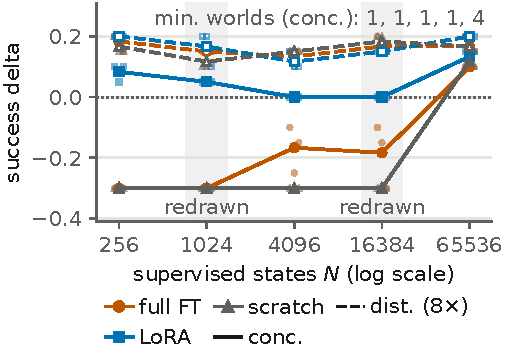
\includegraphics[width=0.98\columnwidth]{figures/fig_c14_dynamic.pdf}
\caption{The matched-label factorial, dynamic substrate (static panel and tables in the appendix): success delta vs.\ the frozen zero-shot source at fixed state count $N$, frozen test cohort, binding budgets; curves connect the five evaluated $N$ levels. Solid: concentrated (fewest worlds supplying $N$; counts annotated); dashed: the same $N$ over $8\times$ as many worlds; small markers: the three adaptation seeds (one sampled world set per cell). Concentrated supervision drops held-out success for full fine-tuning and scratch; distributing the same labels prevents it; recovery at $N{=}65{,}536$ coincides with the world minimum rising to 4. Shaded bands mark $N$ levels with targeted independent world redraws, which preserve positive coverage contrasts there; one redraw LoRA cell degrades (appendix).}
\label{fig:factorial}
\end{figure}

\textbf{Direct contrasts: LoRA retains success at $K{=}1$; full fine-tuning overtakes on effort by $K{=}16$.} At $K{=}1$ the map-paired full-FT$-$LoRA success difference is negative in all six cells (three held-out static targets $\times$ two backbones, HRM and ON-LSTM), with the 95\% interval excluding zero in four (worst $-0.600$ $[-0.773,-0.407]$ on large rooms/HRM). LoRA retains the zero-shot gain (dense maze ratio 0.686, success $+0.467$); full fine-tuning reaches ratio 1.293 on large rooms, and scratch is harmful on dense maze ($-0.167$, interval excluding zero). At $K{=}16$ the contrast reverses on effort: the paired expansion-ratio difference favors full fine-tuning in all six cells, with the map-bootstrap interval excluding zero in five (up to $-0.366$ $[-0.489,-0.235]$). Success is at near-parity (one cell's interval favors full fine-tuning). A 27-cell matched-compute ablation finds bounded and unbounded LoRA nearly identical (maximum map-level ratio delta 0.037), so the output clamp does not explain why LoRA's effort gains stall at higher $K$. LoRA is not universally protective (bugtrap ratio 1.153 by $K{=}32$). Dynamic maps are label-dense ($\sim$15{,}507 supervised states per world), and at dynamic $K{=}1$ full fine-tuning is not systematically catastrophic while LoRA improves on the source rather than merely preserving it. Per-cell contrasts and $K$-indexed curves are in the appendix.

\textbf{A matched-label factorial separates label count from distinct-world coverage.} The $K$-indexed protocol confounds two quantities: adding maps adds labels and worlds together. A preregistered factorial therefore holds the number of supervised states $N$ fixed (256 to 65{,}536 by factors of 4) and varies only whether those states come from the fewest worlds that can supply them (\emph{concentrated}) or from eight times as many (\emph{distributed}). Both domains run under matched optimizer steps (Figure~\ref{fig:factorial}; protocol and tables in the appendix). Each cell adapts one deterministically sampled world set (seeds vary initialization and batch order). The preregistered primary hypothesis (a full-fine-tuning$\times\log N$ effort crossover) is rejected (interaction $-0.0025$ $[-0.0087, +0.0028]$). The coverage readout below is the prespecified secondary endpoint. Concentrated supervision causes a held-out success drop for full fine-tuning and scratch in both domains: $-0.300$ in every seed at dynamic concentrated $N \leq 1{,}024$, and still negative in every seed at $N{=}16{,}384$ from a single world (one of three seeds excludes zero). Distributing the \emph{same} states across more worlds prevents the drop ($+0.15$ to $+0.20$; Figure~\ref{fig:factorial}).

The 30 direct distributed$-$concentrated contrasts (each pairing two of the 60 cells) carry BH-corrected sign-flip tests (added post hoc during review response; appendix). For full fine-tuning and scratch, $q{<}0.05$ in all 10 cells where concentration forces at most two distinct worlds and in none of the 10 where it forces four or more (threshold descriptive). No harmful LoRA interval excludes zero in the original 60 cells (worst $-0.067$ $[-0.167, 0.000]$). Absent a noninferiority margin, this is a failure to observe degradation, not equivalence. Targeted world-draw replications at the key cells preserve the positive coverage direction: all 18 contrasts are positive (scratch excludes zero in all six, full fine-tuning in five of six; one static contrast touches zero). One redraw LoRA cell does degrade, its interval excluding zero (static concentrated $N{=}256$, still the least-degraded method in that cell; appendix). On the static matched expansion ratios (the domain with adequate jointly solved counts), full fine-tuning is at or below LoRA at every tested $N$, consistent with the rejected interaction above. Dynamic effort cells contain one jointly solved map and support no inference. Because ratios condition on solved maps, degraded-success cells can look spuriously efficient. The factorial's conclusions therefore rest on success. Within this factorial, low-rank adaptation's low-supervision advantage appears in \emph{success} and aligns with distinct-world coverage rather than label count.

\section{Scope and Boundary Results}

\textbf{Discrete transfer.} In a separate pooled-multitask study, the pooled HRM base under additive integration improves mean grid success over the Manhattan baseline (0.591$\to$0.612) at lower mean expansions (descriptive; appendix). A 3--8-seed rank-only pilot on selected maps finds 6--15\% expansion reductions at $w{=}1.0$ with equal or higher observed success (no full-suite confirmation).

\textbf{Architecture and hierarchical depth.} Architecture rankings differ across tasks and input representations (the U-Net leads the dynamic field study, the HRM the lowest single-suite dynamic ratio, the ON-LSTM the early scalar stage). In compositional \emph{mission} tasks (waypoint sequences with keys/doors) with oracle-verified headroom for deeper reasoning (appendix), no structured model meets the preregistered depth dose--response criterion, and learned halting moves \emph{opposite} to the depth hypothesis (map-level $\rho{=}-0.578$, permutation $p{=}5\times10^{-5}$). Five of 33 recurrent cells suffer constant-prediction collapse and are excluded from capacity conclusions. Follow-ups on persistent memory, iterative refinement, hierarchical substitution, and persistent search state are also negative (appendix). These negatives are formulation-specific; they do not show that recurrence, memory, or hierarchy are universally ineffective \citep{jolicoeur2025trm,czechowski2021subgoal}.

\textbf{Restricted-observation transfer.} A final static study restricts the model to a radius-0.20 local subgraph, trains it from behavior-derived returns rather than shortest-path labels, and integrates it through one inference-time Bellman backup. The frozen comparison runs on a disjoint 144-map cohort. Its path-quality criterion is comparator-relative, adopted after the original absolute ceiling failed in development (appendix). The local MLP reduces mean per-map expansions against the complete-map field HRM by 12.96 (95\% CI $[-16.30,-9.74]$; 109 wins/3 ties/32 losses) at better path quality (mean/maximum cost ratios 1.024/1.162 versus 1.031/1.335). A separate control, ranking within a $w{=}1.10$ focal band, meets its bounded-suboptimality certificate on all 144 maps. In sequential ablations the point estimate first becomes favorable after the backup (static insertion loses by $+16$; one backup reaches $-1.21$, interval crossing zero; frozen scale calibration then yields the confirmed reduction).
\section{Related Work}

\textbf{Learned guidance for search.} Learned heuristics arise from bootstrapping \citep{arfaee2011bootstrap}, oracle imitation \citep{bhardwaj2017sail}, differentiable search \citep{yonetani2021neuralastar}, grid transformers \citep{kirilenko2023transpath}, classical-planning objectives \citep{ferber2020neural}, and ranking \citep{chrestien2023rank}. We retain classical graph search throughout and jointly evaluate cross-family and dynamic transfer of identical trained models and additive-versus-rank-only integration of the \emph{same} predictions under a shared planner and information set \citep{pohl1970,pearl1982semiadmissible,aine2016mha}.

\textbf{Dynamic, real-time, and motion planning.} The dynamic substrate uses time-expanded space--time search in the spirit of cooperative A\textsuperscript{*} \citep{silver2005cooperative}; safe-interval planning \citep{phillips2011sipp} is a faster alternative, evaluated here as an unbudgeted optimal control. The restricted-observation study relates to real-time heuristic search \citep{korf1990rta,koenig2006rtaa}; its one-step backup resembles a value-iteration-network update \citep{tamar2016vin,lee2018gppn} and neural algorithm execution \citep{velickovic2021nar} but runs once at inference over a radius-bounded subgraph. Learned samplers and end-to-end motion planners \citep{ichter2018sampling,qureshi2019mpnet} replace the planner itself. We keep a fixed classical planner and learn only its guidance on a PRM \citep{kavraki1996prm}.

\textbf{Adaptation and recursive architectures.}\hspace{0.25em}LoRA \citep{hu2021lora}, model soups \citep{wortsman2022soups}, and task arithmetic \citep{ilharco2022task} motivate the low-rank and adapter-interpolation studies (appendix). The contribution is the low-rank-versus-full-rank comparison as a function of label availability and of supervision distribution across worlds. HRM \citep{wang2025hrm}, adaptive computation \citep{graves2016act,banino2021pondernet}, and simplified recursive models \citep{jolicoeur2025trm} motivate the architecture experiments. Our results concern heuristic regression and integration, not their benchmarks.

\section{Limitations}

\textbf{Design and selection.} Most continuous primary results are single-GPU validations with one primary training seed, and several experiments reuse trained bases or test maps. Only the two confirmation cohorts (50-map dynamic, 144-map restricted-observation) are selection-free, and only after development-time choices. Static calibration shares worlds with evaluation (anchor-only). Baselines are the anchor, weighted A\textsuperscript{*}, and SIPP; external \emph{learned} planners are not compared. The grid extension was post hoc. A suite-indexing defect made the original SIPP, extended-grid, wall-time, and residual-probe reference runs evaluate \emph{sibling} cohorts: same-generator cohorts from unintended seed ranges. All were re-executed on the frozen cohort under unchanged rules, identity hash-verified (world manifest and erratum in the appendix; the weighted-A\textsuperscript{*} baseline used the correct cohort).

\textbf{Statistics and coverage.} Matched-effort magnitudes vary by pipeline on three suites. Quoted intervals underrepresent training-run uncertainty (across-pipeline ranges reported). The discrete result covers selected cells. For stages that pooled repeated evaluations, map-clustered reanalysis (appendix) supports the quoted conclusions (not every exploratory table regenerated). The factorial covers one target family per domain, three adaptation seeds, and one sampled world set per cell (targeted redraws in the appendix); coverage counts worlds and does not measure geometric diversity. Matching covers labels and steps, not world-generation cost. Per-cell readouts are marginal (adjusted inference covers the 30 contrasts; the two-world threshold is descriptive). The probe and few-shot analyses are post hoc. Dynamic experiments report expansions rather than end-to-end latency (5-map-per-suite CPU timings; appendix).

\textbf{Scope.} The restricted-observation confirmation is static, one seed and cohort, tests input restriction only, has no formal bound on the primary unbounded comparison, and is slower in wall time. Dynamic obstacles are deterministic. Stochastic motion, kinodynamic constraints, multi-agent coupling, physical robots, and non-2-D settings are untested. The external test coarsens and rectangle-decomposes five source maps, adds synthetic dynamics, and nests instance-level tests in those maps. SIPP's interval unit is not resource-equivalent to $(v,t)$ expansions. Negative results are failures to observe improvement under the tested protocols, not universal rejections.

\section{Conclusion}

Across the tested settings, training formulation and planner integration explained outcomes more consistently than model family: the same model collapses or transfers with its formulation; identical predictions help or fail with their integration. A development-selected blind U-Net, frozen before confirmation, transferred zero-shot: success improved on all six suites and matched expansions fell 73--95\%. Against success-tuned weighted A\textsuperscript{*} the success advantage survives only on spiral, unbudgeted SIPP solves every feasible instance optimally, and the advantage does not reproduce on the five MovingAI-derived maps: the result concerns learned guidance within budgeted time-expanded search, not a faster dynamic planner. In adaptation, distinct-world coverage separates methods: low-rank updates preserve success when worlds are few, full fine-tuning matches success at lower effort with more labeled maps (static $K{=}16$), and distributing a fixed label count across more worlds removes the factorial's concentrated losses.

\bibliography{references}

% AAAI-27 requires the reproducibility checklist to be uploaded separately
% in the designated submission field; it should not be included in this PDF.

\end{document}
